\begin{minipage}{.6\linewidth}
	\begin{flushright}
		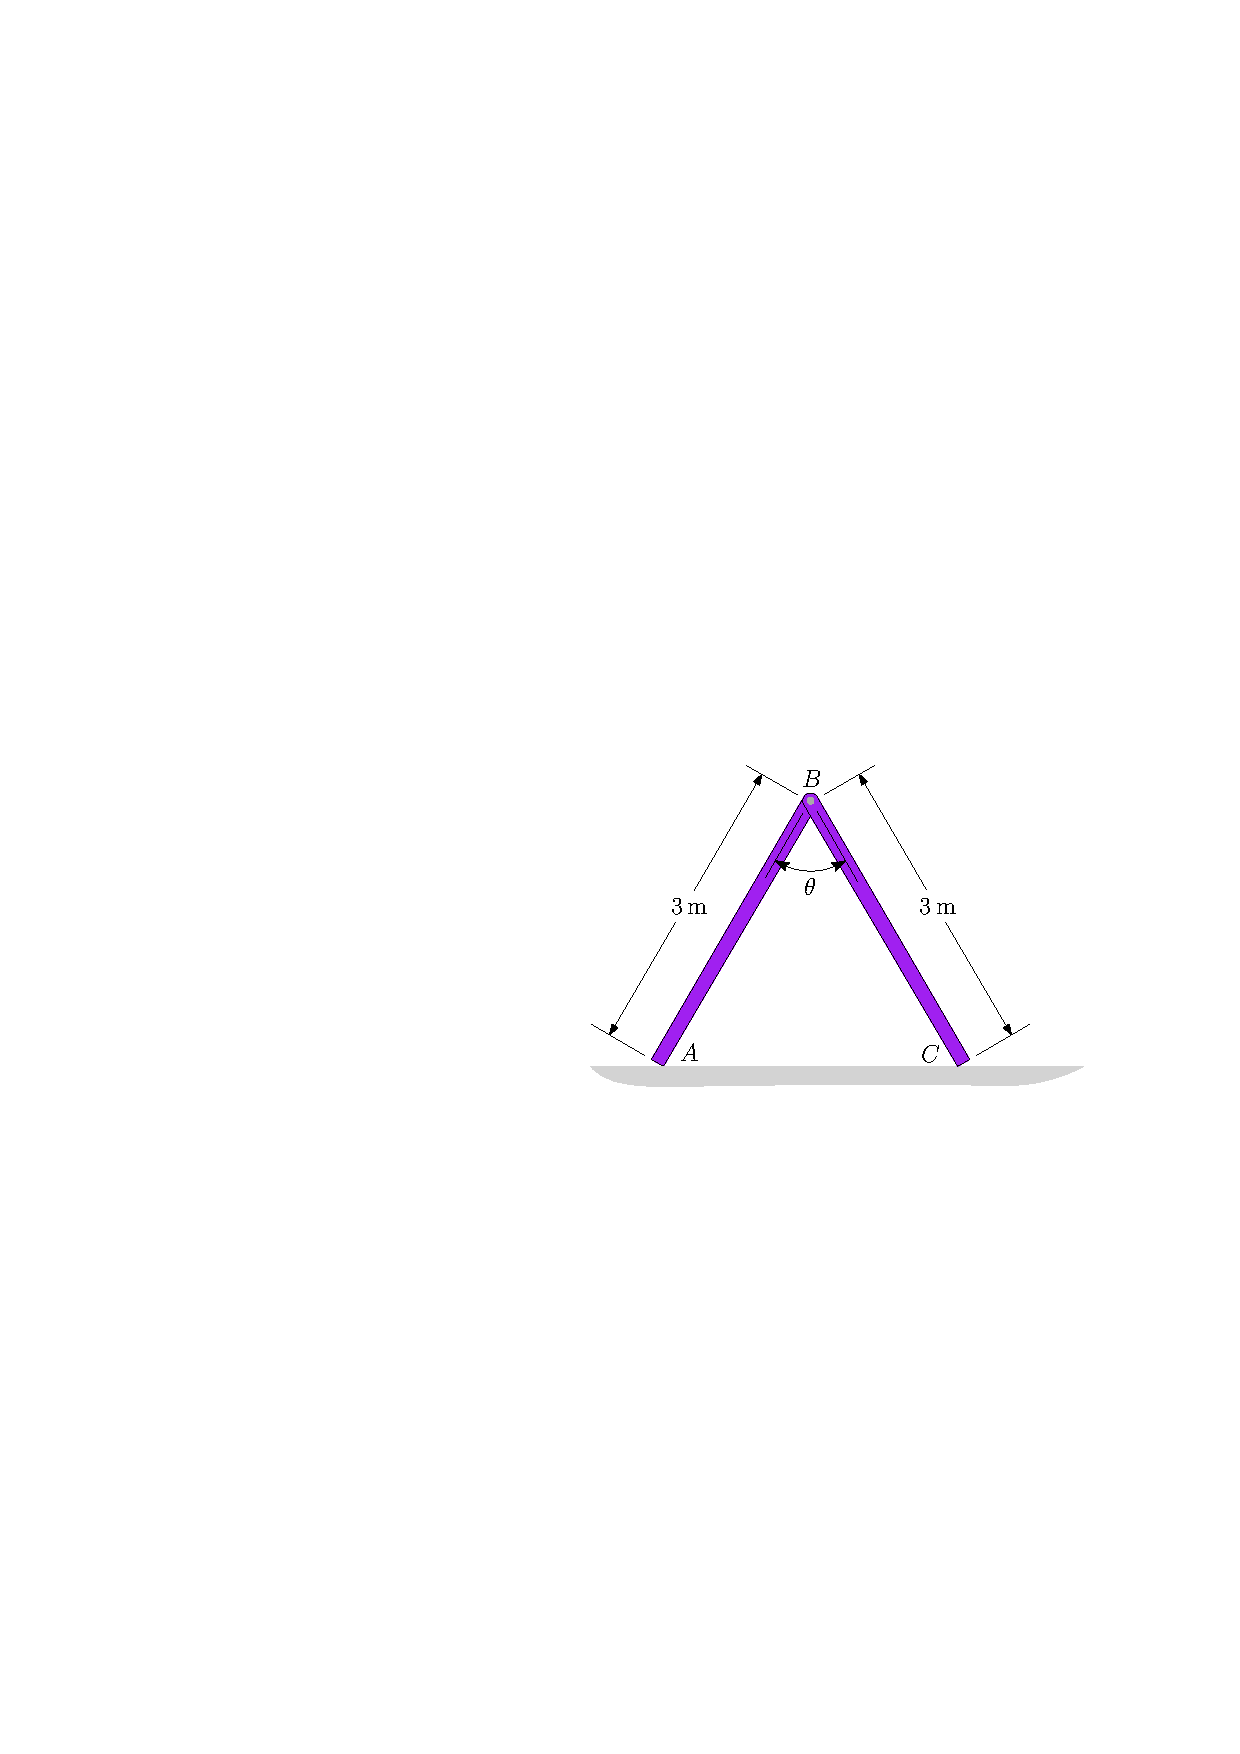
\includegraphics[scale=1.1]{../../images/draw_3_2}
	\end{flushright}
\end{minipage}
\begin{minipage}{.4\linewidth}
	\item Determine a velocidade angular das duas barras de \SI{10}{\kilogram} quando $\theta=\SI{180}{^{\circ}}$, se elas são liberadas do repouso na posição $\theta=\SI{60}{^{\circ}}$. Despreze o atrito.
\end{minipage}